%---------------------------------------------------------------------------------------------
% WORKSHOP IN SEVERAL COMPLEX VARIABLES AND PDE's - Serra Negra                        %
%---------------------------------------------------------------------------------------------

\documentclass[a0,portrait]{a0poster}

%-PACKAGES
%----------------------------------------------------
%\usepackage[latin1]{inputenc}                       %
%\usepackage[brazil]{babel}                          %
\usepackage{multicol}                               %
\usepackage{pdftricks}                              %
\usepackage{color}                                  %
\usepackage{colortbl}                               %
\usepackage{setspace}                               %
\usepackage{amsmath,amsthm,amsfonts,amssymb}        %
\usepackage{type1cm}
%\usepackage{amscd,bezier,amstext,natbib,bm,makeidx} %
%\usepackage{graphicx}                               %
%\usepackage{wrapfig}                                %
%\usepackage{psfrag}                                 %
%\usepackage{float}                                  %
%\usepackage{epsfig}                                 %
%\usepackage[all]{xy}                                %
%----------------------------------------------------
\usepackage{tikz}

\synctex=1 

%-AMBIENTES/ENVIRONMENTS
%----------------------------------------------------
\newtheorem{theorem}{Theorem}
\newtheorem{corollary}[theorem]{Corollary}
\newtheorem{observation}[theorem]{Observation}
\newtheorem{lemma}[theorem]{Lemma} 
%---------------------------------------------------- 

%-FORMAT
%----------------------------------------------------
\setlength{\textwidth}{77.0cm}                      %
\setlength{\textheight}{110.00cm}                   %  
                                                    %
\setlength{\oddsidemargin}{1.0cm}                   %  
\setlength{\topmargin}{1.0cm}                       %  
                                                    %
\setlength{\columnsep}{0.7cm}                       %  
\setlength{\parindent}{0cm}                         %
%-------------------------------------------------------------------------------------------------------
\newcommand{\ds}{\displaystyle}
\newcommand{\ts}{\textstyle}
\newcommand{\nin}{\noindent}
\newcommand{\rr}{\mathbb{R}}
\newcommand{\nn}{\mathbb{N}}
\newcommand{\zz}{\mathbb{Z}}
\newcommand{\cc}{\mathbb{C}}
\newcommand{\ci}{\mathbb{T}}
\newcommand{\zzdot}{\dot{\zz}}
\newcommand{\wh}{\widehat}
\newcommand{\p}{\partial}
\newcommand{\ee}{\varepsilon}
\newcommand{\vp}{\varphi}
\newcommand{\wt}{\widetilde}

%-------------------------------------------------------------------------------------------------------
\begin{document}
\begin{center}

      \fontsize{76}{1}\textbf{\textcolor{blue}{VI Workshop on Geometric Analysis of PDE and Several Complex Variables}}


 \end{center}

 \vspace{1.0cm}

 \begin{center}

      \fontsize{66}{1}\textbf{{Continuity Properties of the Solution Map for the Hyperelastic Rod Equation}}

 
 \end{center}

 \vspace{1.0cm}

 \begin{center}

    \begin{center}
     {\huge  David Karapetyan} 
    \end{center}

 \end{center}
\vspace{1.0cm}
 

    \begin{center}
     {\large August 3, 2011}
    \end{center}
 

   \vspace{1.8cm}

   \setlength{\columnsep}{2.5cm}  
   
   
   \begin{multicols}{3}

      \baselineskip=1.6em
%LOGO
     % 
     %\vspace{1.0 cm}
     %\hspace{1.0 cm}
     %\begin{picture}(27.9,11.9)
     %\put(15.5,5){\includegraphics[scale=2.0]{logo.jpg}}
     %\end{picture}



\vspace{-2.0 cm}

%-------------------------------------------------------------------------------------------------------





\section*{\center{{Abstract}}}


It is proved that for $s > 3/2$
the data-to-solution map for the hyperelastic rod (HR) equation is not uniformly
continuous in Sobolev spaces with exponent $s$. Since HR is well-posed in Sobolev
spaces for $s > 3/2$ with continuous dependence on initial data, this result shows
that continuity is optimal. Furthermore, we show that the solution map is H\"older
in $H^s$ if the norm is replaced with a weaker $H^r$ norm.
%-------------------------------------------------------------------------------------------------------
 




\section*{\center{{Introduction}}}


We consider the hyperelastic rod (HR) Cauchy problem
\begin{gather}
 \p_t u =  -\gamma u \p_x u -
 \p_{x} D^{-2} \left[ \frac{3-\gamma}{2}u^2 +
\frac{\gamma}{2} \left( \p_x u \right)^2
\right],
\label{hyperelastic-rod-equation}
\\
 u(x,0) = u_0(x), \; \; x \in \rr, \; \; t \in \rr
\label{init-cond}
\end{gather}
%
%
where 
\begin{equation*}
	D^{m} = (1 - \p_x^2)^{m/2}, \quad m \in \rr
\end{equation*}
and  $\gamma$  is a  nonzero constant. The HR equation was first
derived by Dai in \cite{Dai_1998_Model-equations} as a one-dimensional 
model for finite-length and
small-amplitude axial deformation waves in thin cylindrical
rods composed of a compressible Mooney-Rivlin
material. The derivation relied upon a reductive perturbation technique, 
and took into account the nonlinear dispersion of pulses propagating 
along a rod. It was assumed that each cross-section of the rod is 
subject to a stretching and rotation in space. The solution $u(x,t)$ to the 
HR equation represents the radial stretch relative
to a pre-stressed state, while $\gamma$ is a fixed constant depending upon 
the pre-stress and the material used in
the rod, with values ranging from $- 29.4760$ to $3.4174$.
%
\\
\\
The well-posedness of the HR equation has been studied by several authors. 
In Yin \cite{Yin_2003_On-the-Cauchy-p} and Zhou 
\cite{Zhou_2005_Local-well-pose}, a proof of local well-posedness in Sobolev 
spaces $H^s$,  $s > 3/2$, is described  on the line and the circle, respectively. 
Their approach is to rewrite the HR equation   
in its non-local form, and then to verify the conditions needed to apply 
Kato's semi-group theory \cite{Kato_1975_Quasi-linear-eq}. Using an alternative,
Galerkin type method outlined in Taylor \cite{Taylor_1991_Pseudodifferent}, local
well-posedness in Sobolev spaces $H^s$,  $s > 3/2$ on the line and the circle is
established in \cite{Karapetyan:2010fk}. 
For details on how this is done for CH ($\gamma =1$) on the line, see Rodriguez-Blanco 
\cite{Rodriguez-Blanco_2001_On-the-Cauchy-p}. Blow-up criteria 
is also investigated in \cite{Yin_2003_On-the-Cauchy-p} and 
\cite{Zhou_2005_Local-well-pose}, as well as by Constantin and Strauss 
\cite{Constantin_2000_Stability-of-a-}. 
\\
\\
Setting $\gamma = 0$ gives the celebrated 
BBM equation, which was proposed by 
Benjamin, Bona, and Mahony 
\cite{Benjamin_1972_Model-equations} as a model for 
the unidirectional evolution of long waves.
Solitary-wave solutions to this 
equation are global and orbitally stable (see Benjamin 
\cite{Benjamin_1972_The-stability-o}, 
\cite{Benjamin_1972_Model-equations}, and 
\cite{Constantin_2000_Stability-of-a-}).
For more general $\gamma$, the existence of global 
solutions to HR on the line with constant $H^1$ energy
was proved recently by Mustafa \cite{Mustafa_2007_Global-conserva}
using the approach developed by Bressan and 
Constantin in \cite{Bressan_2007_Global-conserva}. Using a vanishing 
viscosity argument, Coclite, 
Holden, and Karlsen \cite{Coclite_2005_Global-weak-sol}
established existence of a strongly continuous semigroup of global 
weak solutions of HR on the line for initial data in $H^1$.
Bendahmane, Coclite, and Karlsen 
\cite{Bendahmane_2006_Hsp-1-perturbat} extended this result to traveling 
wave solutions that are supersonic solitary shockwaves.
For more information on the existence of global solutions to the HR
equation, see Holden and Raynaud \cite{Holden_2007_Global-conserva}
and \cite{Yin_2003_On-the-Cauchy-p}. 
\\
\\
There is a variety of traveling wave solutions to the HR equation that can be 
obtained using various combinations of peaks, cusps, compactons, 
fractal-like waves, and plateaus (see Lenells 
\cite{Lenells_2006_Traveling-waves}). Orbital stability of solitary wave 
solutions was proved in \cite{Constantin_2000_Stability-of-a-}.
Solitary shock wave formation was 
analyzed in Dai and Huo \cite{Dai_2000_Solitary-shock-} using traveling 
wave solutions of the HR equation to derive a system of ordinary differential 
equations, with a vertical singular line in the phase plane corresponding with the 
formation of shock waves. Head-on collisions between two solitary 
waves was investigated in the work of Hui-Hui Dai, 
Shiqiang Dai, and Huo \cite{Dai_2000_Head-on-collisi} using a reductive 
perturbation method coupled with the technique of strained coordinates. 
\section*{\center{{Main Results}}}


We are interested in the continuity properties of the data-to-solution map for the HR 
equation. 
%
%%%%%%%%%%%%%%%%%%%%%%%%
%
%
%    Theorem:  hr-non-unif-dependence
%
%
%%%%%%%%%%%%%%%%%%%%%
%
\begin{theorem}
\label{hr-non-unif-dependence}
Let $\gamma$ be a nonzero constant. Then 
the data-to-solution map $u(0) \mapsto u$ of the Cauchy-problem
for the HR equation
\eqref{hyperelastic-rod-equation}-\eqref{init-cond}
is not uniformly continuous
from any bounded subset of  $H^s$ into $C([-T, T], H^s)$
for $s>3/2$ on the line and on the circle.
%
\end{theorem}
%
%
%
%
The approach for proving Theorem \ref{hr-non-unif-dependence}  
mirrors  that in Himonas and Kenig \cite{Himonas:2009fk} and 
Himonas, Kenig, and Misiolek \cite{Himonas_2009_Non-uniform-dep-per}.
That is, we choose 
approximate solutions to the HR equation such that the size of the difference between approximate and actual solutions with 
identical initial data is negligible. Hence, to understand the degree of 
dependence, it suffices to focus on the behavior of the approximate 
solutions (which are simple in form), rather than on the behavior of the 
actual solutions. In order for the method to go through, we 
need well-posedness estimates for  the size of the 
actual solutions to the HR equation, as well as
lower bound for their lifespan. This permits us to obtain an upper 
bound for the size of the difference of approximate and actual solutions. 
More precisely, we prove the following well-posedness result with estimates,  
stated in both the periodic and non-periodic case:


%%%%%%%%%%%%%%%%%%%%%%%%
%
%            wp of theorem in R and T
%
%%%%%%%%%%%%%%%%%%%%%%%%
%
%
%
%
\begin{theorem}
\label{thm:HR_existence_continuous_dependence}
If   $s>3/2$  then we have:

(i) If $u_0\in H^s$  then  there exists a unique solution to
the Cauchy problem  \eqref{hyperelastic-rod-equation}--\eqref{init-cond} in $C([-T, T], H^s)$, where 
the lifespan  $T$ depends on the size
of the initial data $u_0$. Moreover, 
the  lifespan $T$ satisfies the lower bound estimate 
%
%
%
\begin{equation*}
T
\ge
\frac{1}{2c_s \|u_0\|_{H^s}}.
\end{equation*}
%

(ii)
The data to solution map $u_0 \mapsto u$ is continuous from
bounded sets of $H^s$ into  $C([-T, T], H^s)$,
and the solution $u$ satisfies the estimate
%
%
\begin{equation*}
\|
u(t)
\|_ {H^s}
\le
2
\|
u_0
\|_{H^s}, \ \ |t|\le T.
\end{equation*}
%
%
%
\end{theorem}
The preceding results can be found in \cite{Karapetyan:2010fk}. Expanding on
this work, we study the continuity properties of the data-to-solution map for HR
in weaker topologies. More precisely, motivated by \cite{Chen:2011fk}, we show the following result:
%
\begin{theorem}
  For $\gamma \neq 0$, the
  data to solution map for HR is H\"older continuous from $B_{H^{s}}(R)$ (in
  the topology of $H^{r}$) to $C([0, T], H^{r})$, where $T = T(R)$, for $s >
  3/2$, $-1 \le r < s$. More
  precisely, decompose the set $\Omega = \left\{ (s, r) \in \rr^{2}  \right\}$
  into the pieces
  %
  %
  \begin{equation*}
  \begin{split}
    & \Omega_{1} = \left\{ (s, \ r):  \ s < 3/2 \right\}
    \\
    & \Omega_{2} = \left\{ (s, \ r):
     \ s>3/2, \ r < -1  \right\}
    \\
    & \Omega_{3} = \left\{ (s, \ r):
     \ s>3/2, \ r > s  \right\}
    \\
    & \Omega_{4} = \left\{ (s, \ r):
     \ s>3/2, \ -1 \le r \le s-1, \ s + r \ge 2  \right\}
    \\
    & \Omega_{5} = \left\{ (s, \ r):
     \ s>3/2, \ -1 \le r < 2-s \right\}
    \\
    & \Omega_{6} = \left\{ (s, \ r):
    \  s>3/2, \  s-1 < r < s  \right\}.
    \end{split}
\end{equation*}
  %
  %
\label{thm:main-thm}
\end{theorem}
%
\begin{center}
\begin{tikzpicture}[scale=4]
% Draw thin grid lines with color 40% gray + 60% white

% Draw x and y axis lines
\draw [->] (0,0) -- (3,0) node [below] {$s$};
\draw [->] (0,-2) -- (0,3) node [left] {$r$};
\draw [->, dashed] (0,0) -- (3,3) ;
\draw [->, dashed] (0,-1) -- (3,2) ;
\draw [->, dashed] (0,2) -- (3,-1) ;
\draw [->, dashed] (0,-1) -- (3,-1) ;
\draw [->, dashed] (3/2,-2) -- (3/2, 3);
\fill[color=green, fill opacity=0.3] (1.5, 0.5) -- (3,2) -- (3,0) -- (3,-1);
\fill[color=red, fill opacity=0.3] (1.5, 0.5) -- (1.5,1.5) -- (3,3) -- (3,2);
\fill[color=yellow, fill opacity=0.3] (0, -2) -- (1.5, -2) -- (1.5, 3) -- (0, 3);
\fill[color=blue, fill opacity=0.3] (1.5, 0.5) -- (1.5, -1) -- (3, -1);
\fill[color=brown, fill opacity=0.3] (1.5, 1.5) -- (3, 3) -- (1.5, 3);
\fill[color=cyan, fill opacity=0.3] (1.5, -1) -- (3, -1) -- (3, -2) -- (1.5, -2);


\foreach \x/\xtext in { 1, 2}
    \draw[shift={(\x,0)}]  node[below] {$\xtext$};
\foreach \y/\ytext in {-1, 1, 2}
    \draw[shift={(0,\y)}]  node[left] {$\ytext$};
    \draw (1,0.5) node {$\Omega_{1}$};
    \draw (2,2.5) node {$\Omega_{3}$};
    \draw (2,1.5) node {$\Omega_{6}$};
    \draw (2,-1.5) node {$\Omega_{2}$};
    \draw (2,0.5) node {$\Omega_{4}$};
    \draw (2,-0.5) node {$\Omega_{5}$};
\end{tikzpicture}
\end{center}
%
%
Then for two initial data $u_{0}, v_{0} \in B_{H^{s}}(R)$, there exist unique
corresponding solutions $u(x,t), v(x,t)$ for $0 \le t \le T= T(R)$ to the
HR equation \eqref{hyperelastic-rod-equation} which satisfy 
%
%
\begin{equation*}
\begin{split}
  \| u(t) - v(t) \|_{H^{r}} \le C \| u_{0} - v_{0} \|^{\alpha(s, r, \gamma)},
  \quad 0
  \le t \le T
\end{split}
\end{equation*}
%
%
where 
%
%
\begin{equation*}
\begin{split}
\alpha = 
\begin{cases}
   1, \quad & (s,r, \gamma) \in \Omega_{4} 
  \\
   2(s-1)/(2-r),  \quad & (s, r, \gamma) \in \Omega_{5}
  \\
   s-r, \quad & (s, r, \gamma) \in \Omega_{6}.
\end{cases}
\end{split}
\end{equation*}

%
%%%%%%%%%%%%%%%%%%%%%%%%%%%%%%%%%%%%%%%%%%%%%%%%%%%%%
%
%
%                Main theorem
%
%
%%%%%%%%%%%%%%%%%%%%%%%%%%%%%%%%%%%%%%%%%%%%%%%%%%%%%
%
%
We remark that this result improves upon the H\"older continuity result in
\cite{Chen:2011fk} (there it is for $0 \le r < s$) by a full degree in $r$. 


%-------------------------------------------------------------------------------------------------------------

\section*{\center{{Outline of Proof of Theorem \ref{thm:main-thm}}}}
%
%
The proof in the periodic case is analogous to that in the non-periodic case.
Hence, we restrict our attention to the non-periodic case. 
%
\subsection*{Region $\Omega_{1}$} 
\label{ssec:reg-2}
This is open. In particular, well-posedness of HR must be proved or disproved
below $3/2$ before we can even consider discussing H\"older continuity in weak
topologies.
\subsection*{Region $\Omega_{2}$} 
\label{ssec:reg-6}
Open. The lower bound on $r$ comes from Lemma \ref{cor1}. Perhaps the lemma can
be strengthened.
\subsection*{Region $\Omega_{3}$} 
\label{ssec:reg-7}
It makes little sense to talk about this region, 
i.e. we assume a priori that our initial
data is in $H^{s}$. 
%
\subsection*{Region $\Omega_{4}$} 
\label{ssec:reg-m-imp}
%
%
Let $u_{0}(x), v_{0}(x)
\in B_{H^{s}}(R)$, $s > 3/2$ be two initial datum. Then from
the well-posedness theory for HR \cite{Karapetyan:2010fk}, we
know that there exists unique corresponding solutions $u, v \in C(I,
B_{H^{s}}(2R))$ to \eqref{hyperelastic-rod-equation}.
Set $v=u-w$. Then $v$ solves the Cauchy-problem
%
%
\begin{align}
	\label{uniqueness-exp}
& \p_t v
=  -\frac{\gamma}{2} \p_x [v(u + w)] 
\\
\notag
& \phantom{\p_t v = }- D^{-2} \p_x \left\{
\frac{3-\gamma}{2}[v(u+w)] + \frac{\gamma}{2}[\p_x v \cdot \p_x (u+w)]
\right\},
\\
& v(x,0) = u_{0}(x) - v_{0}(x).
\label{uniqueness-init-data}
\end{align}
%
%
%
%
Applying $D^r$ to both sides of \eqref{uniqueness-exp}, then 
multiplying both sides by $D^r v$ and integrating, we obtain
%
%
\begin{equation*}
\begin{split}
 \frac{1}{2} \frac{d}{dt} \|v\|_{H^r}^2
 = & -\frac{\gamma}{2} \int_{\rr} D^r \p_x [v(u+w)] \cdot
D^r v \ dx
\\
& - \frac{3-\gamma}{2} \int_{\rr}  D^{r -2}
\p_x[v(u+w)] \cdot
D^r v \ dx  
\\
& - \frac{\gamma}{2} \int_{\rr} D^{r 
-2} \p_x [ \p_x v
\cdot \p_x (u+w)]\cdot D^r v \ dx .
\end{split}
\end{equation*}
%
%
We estimate the right hand side using a series of key lemmas.
%
\begin{lemma}[\cite{Himonas_2009_Non-uniform-dep-per}]
\label{cor1}
If $s > 3/2$ and $-1 \le r  \le s -1$, then
%
%
\begin{equation*}
\begin{split}
\|[D^r \p_x ,f]g\|_{L^2} \le C \|f\|_{H^s} \|g\|_{H^r}.
\end{split}
\end{equation*}
%
%
\end{lemma}
%
%
%
%
\begin{lemma}
For $s > 3/2$, $r \le s$, $s + r \ge 2$, we have
%
%
\begin{equation*}
\begin{split}
  \| fg \|_{H^{r-1}} \le \| f \|_{H^{r-1}} \| g \|_{H^{s}}.
\end{split}
\end{equation*}
%
%
\label{lem:frac-deriv}
\end{lemma}
%
%
%
%
%
%
%
%
%
\begin{lemma}
\label{impo}
If  $s > 3/2$, $r \le s$, and $s + r \ge 2$,  then
%
%
\begin{equation*}
\begin{split}
  \|f_{x}g_{x}\|_{H^{r - 1}} \le C \|f\|_{H^{r}}
\|g\|_{H^{s}}.
\label{11}
\end{split}
\end{equation*}
%
%
\end{lemma}
%
Applying the above lemmas, we get 
%
%
%
\begin{equation*}
\begin{split}
\frac{1}{2} \frac{d}{dt}
\|v\|_{H^r}^2
& \lesssim \|u+w\|_{H^s}
\|v\|_{H^r}^2, \quad | t | < T
\\
& \le 2R \| v \|_{H^{r}}^{2}.
\end{split}
\end{equation*}
%
%
%
%
%
%
%
which implies
%
%
\begin{equation}
  \label{lip-ineq}
\begin{split}
  & \| u(t) - w(t) \|_{H^{r}} \le C \| u_{0} - w_{0} \|_{H^{r}}, 
  \\
  & \text{for} \ | t | < T,
  \ s > 3/2, \ -1 \le r \le s-1, \ s + r \ge 2.
\end{split}
\end{equation}
%
Hence, in region $\Omega_{4}$, the data to solution map is locally Lipschitz from
$B_{H^{s}(R)}$ (in the $H^{r}$
topology) to $C([-T, T], H^{r})$, with Lipschitz constant $C = C(s, r, R)$.
%
%
%
%
%
%
%
%
%
%
\subsection*{Region $\Omega_{5}$} 
\label{ssec:case-4}
%
%
Note that   $-1 \le 2-s \le s-1$ for $s>3/2$ and $s + (2-s) = 2$.
Hence, applying \eqref{lip-ineq}, we bound 
%
%
%
%
\begin{equation}
  \label{fgh}
\begin{split}
  \| v(t) \|_{H^{r}}
  & \le \|v(t) \|_{H^{2-s}}
  \\
  & \lesssim \|v(0) \|_{H^{2-s}}.
  \end{split}
\end{equation}
%
We need the following interpolation
result. 
%
%
%%%%%%%%%%%%%%%%%%%%%%%%%%%%%%%%%%%%%%%%%%%%%%%%%%%%%
%
%
%                interp
%
%
%%%%%%%%%%%%%%%%%%%%%%%%%%%%%%%%%%%%%%%%%%%%%%%%%%%%%
%
%
\begin{lemma}
  For $m_{1} < m < m_{2}$,
  %
  %
  \begin{equation*}
  \begin{split}
    \| f \|_{H^{m}} \le \| f \|_{H^{m_{1}}}^{(m_{2}-m)/(m_{2} - m_{1})} \| f
    \|_{H^{m_{2}}}^{(m -m_{1})/(m_{2} - m_{1})}.
  \end{split}
  \end{equation*}
  %
  %
  %
  %
   %
  %
\label{lem:interp}
\end{lemma}
%
Applying the lemma with $m_{1} =r$, $m = 2-s$, and $m_{2} = s$, we bound the
right hand side of \eqref{fgh} by
%
%
\begin{equation*}
\begin{split}
  \| v(0) \|_{H^{r}}^{\frac{2(s-1)}{2-r}} \|v(0)
  \|_{H^{s}}^{\frac{2-s-r}{s-r}}
  & = \| u_{0} - w_{0} \|_{H^{r}}^{\frac{2(s-1)}{2-r}} \|u_{0} - w_{0}
  \|_{H^{s}}^{\frac{2-s-r}{s-r}}
  \\
  & \lesssim \| u_{0} - w_{0} \|_{H^{r}}^{\frac{2(s-1)}{2-r}}.
\end{split}
\end{equation*}
%
We conclude that
%
%
\begin{equation*}
\begin{split}
  \| u(t) - w(t) \|_{H^{r}} \lesssim \|u_{0} - w_{0} \|_{H^{r}}^{\frac{2(s-1)}{2-r}}.
\end{split}
\end{equation*}
%
%
%
%
\subsection*{Region $\Omega_{6}$} 
\label{ssec:case-2}
%
%
Applying Lemma \ref{lem:interp} and the fact that 
%
%
\begin{equation*}
\begin{split}
  \|v\|_{H^{s}} = \|u - w \|_{H^{s}} \le 4R
\end{split}
\end{equation*}
%
%
we obtain
%
%
\begin{equation}
  \label{pre-lip-ap}
\begin{split}
  \| v(t) \|_{r} & \lesssim \| v(t) \|_{H^{s-1}}^{s-r} \|v(t) \|_{H^{s}}^{1-s+r}
  \\
  & \simeq \| v(t) \|_{H^{s-1}}^{s-r}.
\end{split}
\end{equation}
%
%
Notice that $-1 \le s-1 \le s-1$, and $s + (s-1) = 2s-1 \ge 2$ for $s >3/2$.
Hence, we may apply \eqref{lip-ineq} to bound the right hand side of
\eqref{pre-lip-ap} by
%
%
\begin{equation*}
\begin{split}
  C \|v(0) \|_{H^{s-1}}^{s-r}
  & \lesssim \|v(0) \|_{H^{r}}^{s-r} 
  = \|u_{0} - w_{0}\|_{H^{r}}^{s-r}.
\end{split}
\end{equation*}
%
%
This completes the proof of Theorem \ref{thm:main-thm}. \qed
 
%--------------------------------------------------------------------------------------------------------------

\section*{\center{{Acknowledgment}}}

The author thanks his advisor Alex Himonas for 
his guidance and many helpful remarks. The author also thanks the Department of 
Mathematics at the University of Notre Dame and the Arthur J. Schmitt Foundation for 
supporting his doctoral 
studies.

 
%--------------------------------------------------------------------------------------------------------------



%----------------------------------------------------------------------------------------------------------------------
\end{multicols}
\bibliographystyle{amsalpha-custom}
\bibliography{/Users/davidkarapetyan/math/bib-files/references}

\end{document} 
